\documentclass[crop, tikz]{standalone}
\usepackage{tikz}
\usepackage{bm}

\usetikzlibrary{positioning, matrix}

\tikzset{ 
	tablet/.style={
		matrix of nodes,
		row sep=-\pgflinewidth,
		column sep=-\pgflinewidth,
		nodes={rectangle,draw=black,text width=1.25ex,align=center},
		text height=1.25ex,
		text depth=0ex,
		nodes in empty cells
	},
	texto/.style={font=\footnotesize\sffamily},
	title/.style={font=\small\sffamily}
}

\begin{document}
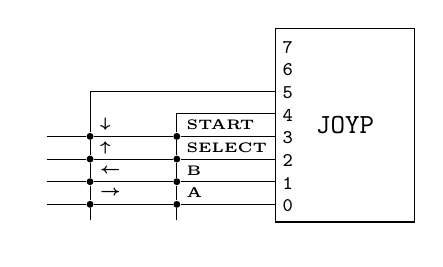
\begin{tikzpicture}[node distance=3cm, auto]
	\node [rectangle, draw, minimum width=5em, minimum height=7em] (joyp) {\tt JOYP};
	\matrix[tablet, draw=none, nodes={draw=none, inner sep = 0.16em}, inner sep=0.1em, left = -0.35cm of joyp] (pt) 
	{
		\node (17){\scriptsize\tt 7}; \\ \node(16){\scriptsize\tt 6}; \\ \node(15){\scriptsize\tt 5}; \\ \node(14){\scriptsize\tt 4}; \\ \node(13){\scriptsize\tt 3}; \\ \node(12){\scriptsize\tt 2}; \\ \node(11){\scriptsize\tt 1}; \\ \node(10){\scriptsize\tt 0};\\
	};	
	
	\node [circle, inner sep=0, minimum size=0.25em, fill=black, left = 1.2cm of 10] (a) {};
	\node [circle, inner sep=0, minimum size=0.25em, fill=black, left = 1.2cm of 11] (b) {};
	\node [circle, inner sep=0, minimum size=0.25em, fill=black, left = 1.2cm of 12] (select) {};
	\node [circle, inner sep=0, minimum size=0.25em, fill=black, left = 1.2cm of 13] (start) {};
	
	\node [circle, inner sep=0, minimum size=0.25em, fill=black, left = 1cm of a] (right) {};
	\node [circle, inner sep=0, minimum size=0.25em, fill=black, left = 1cm of b] (left) {};
	\node [circle, inner sep=0, minimum size=0.25em, fill=black, left = 1cm of select] (up) {};
	\node [circle, inner sep=0, minimum size=0.25em, fill=black, left = 1cm of start] (down) {};
	
	\node [left = 0.5cm of right] (ra) {};
	\node [left = 0.5cm of left] (lb) {};
	\node [left = 0.5cm of up] (usel) {};
	\node [left = 0.5cm of down] (dst) {};
	
	\node [below = 0.15cm of a] (aa) {};
	\node [below = 0.15cm of right] (rr) {};
	
	\draw (ra) -- (right) -- (a) -- (10);
	\draw (lb) -- (left) -- (b) -- (11);
	\draw (usel) -- (up) -- (select) -- (12);
	\draw (dst) -- (down) -- (start) -- (13);
	
	\draw (aa) -- (a) -- node[right] {\tiny\bf A} (b) -- node[right] {\tiny\bf B} (select) -- node[right] {\tiny\bf SELECT} (start) |- node[pos=0.2, right] {\tiny\bf START} (14);
	\draw (rr) -- (right) -- node[right] {\tiny $\bm{\rightarrow}$} (left) -- node[right]{\tiny $\bm{\leftarrow}$} (up) -- node[right]{\tiny $\bm{\uparrow}$} (down) |- node[pos=0.1, right]{\tiny $\bm{\downarrow}$} (15);
\end{tikzpicture}
\end{document}
